\section{Manual de usuario}

\subsection{Introducción} 
Se ha integrado en la aplicación JMR nuevas funcionalidades que permiten generar imágenes a partir de descripciones textuales de forma sencilla y eficiente. Con estas funcionalidades, puedes:
\begin{itemize}
    \item Elegir la fuente de generación de imágenes, ya sea un modelo local o una API online.
    \item Generar imágenes directamente desde descripciones en lenguaje natural.
    \item Consultar en la base de datos imágenes similares a las generadas.
    \item Consultar un historial de imágenes generadas previamente.
    \item Consultar en la base de datos imágenes similares a un prompt.
\end{itemize}

Este manual proporciona una guía paso a paso para utilizar esta funcionalidad, e incluye ejemplos prácticos y una descripción detallada de cada acción disponible en la interfaz.

\subsection{Inicio de la aplicación}
\begin{enumerate}
    \item Abre la aplicación JMR haciendo clic en el icono correspondiente en tu escritorio o desde el menú de inicio de tu sistema operativo.
    \item Una vez abierta, observarás la interfaz principal de JMR, donde se encuentran las dos nuevas funcionalidades de generación de imágenes.
\end{enumerate}

\begin{figure}[H]
    \centering
    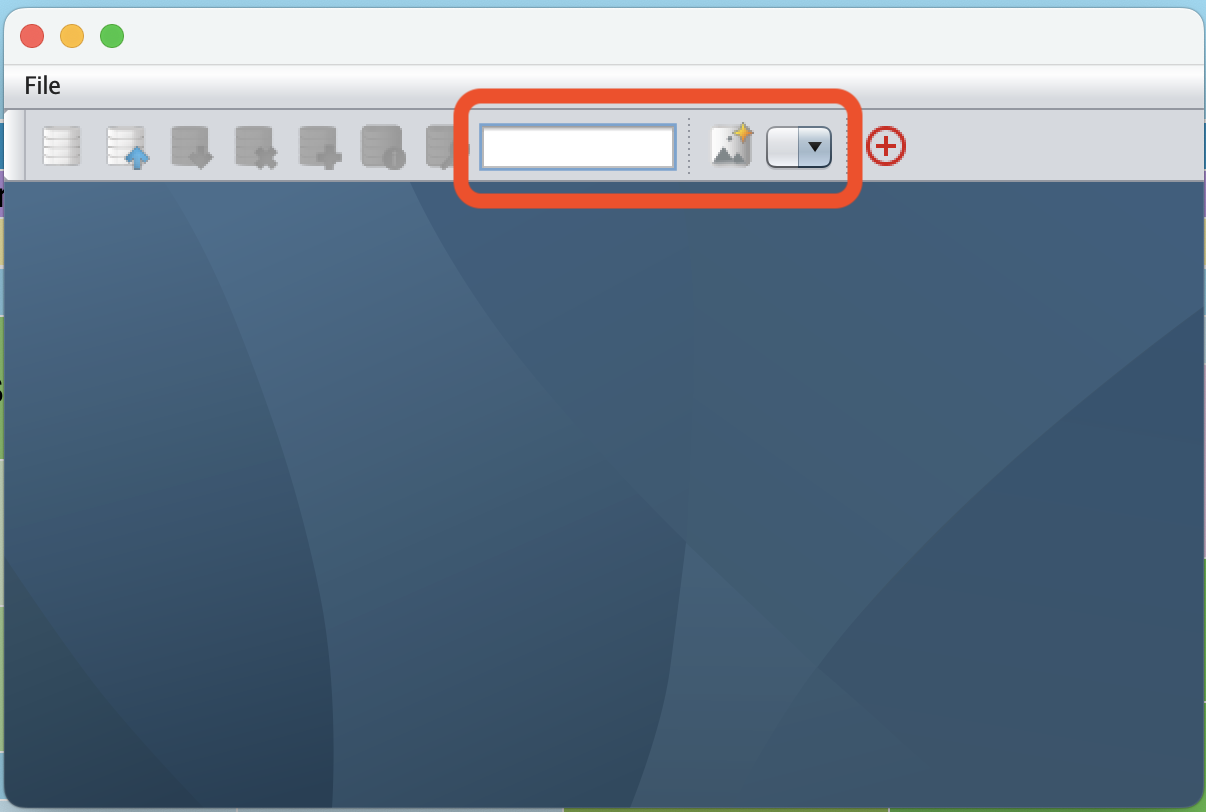
\includegraphics[width=0.5\textwidth]{manual/captura1.png}
    \caption{Inicio de la aplicación con las dos nuevas funcionalidades}
    \label{fig:inicio}
\end{figure}

\subsection{Descripción de la interfaz} 
Las nuevas funcionalidades de generación de imágenes están integradas en la barra superior y presentan los siguientes elementos:
\begin{enumerate}
    \item \textbf{Elección de API}: Un menú desplegable que permite seleccionar entre la API local o una API online para la generación de imágenes.
    \item \textbf{Cuadro de texto}: Espacio donde puedes escribir la descripción textual de la imagen que deseas buscar en la base de datos.
    \item \textbf{Generar imagen}: Abre una ventana con un área de texto en la que puedes describir la imagen a generar. Dentro de esta hay un botón para generar y visualizar la imagen descrita.
    \item \textbf{Lista desplegable}: Lista desplegable que muestra un historial de las imágenes generadas junto a sus descripciones. Permite seleccionar una entrada anterior para visualizarla nuevamente.
\end{enumerate}


\subsection{Selección de API para generación de imágenes}

El sistema permite elegir entre dos modos de conexión para la generación de imágenes: utilizando un modelo alojado localmente en el dispositivo, o bien accediendo a una API online como la de Hugging Face. Esta flexibilidad permite al usuario adaptar el sistema a diferentes contextos de uso.

\paragraph{\textbf{Modo de selección}} \mbox{}\\[0.5em]
En la barra superior de la aplicación se encuentra un menú llamado \texttt{API}. Al hacer clic sobre él, se despliega un submenú con las siguientes opciones:

\begin{itemize}
\item \textbf{Local API}: utiliza el modelo alojado en el sistema local (por defecto).
\item \textbf{Online API}: permite realizar peticiones a un servicio externo. Es necesario introducir un token de autenticación para acceder a esta opción.
\end{itemize}

\begin{figure}[H]
\centering
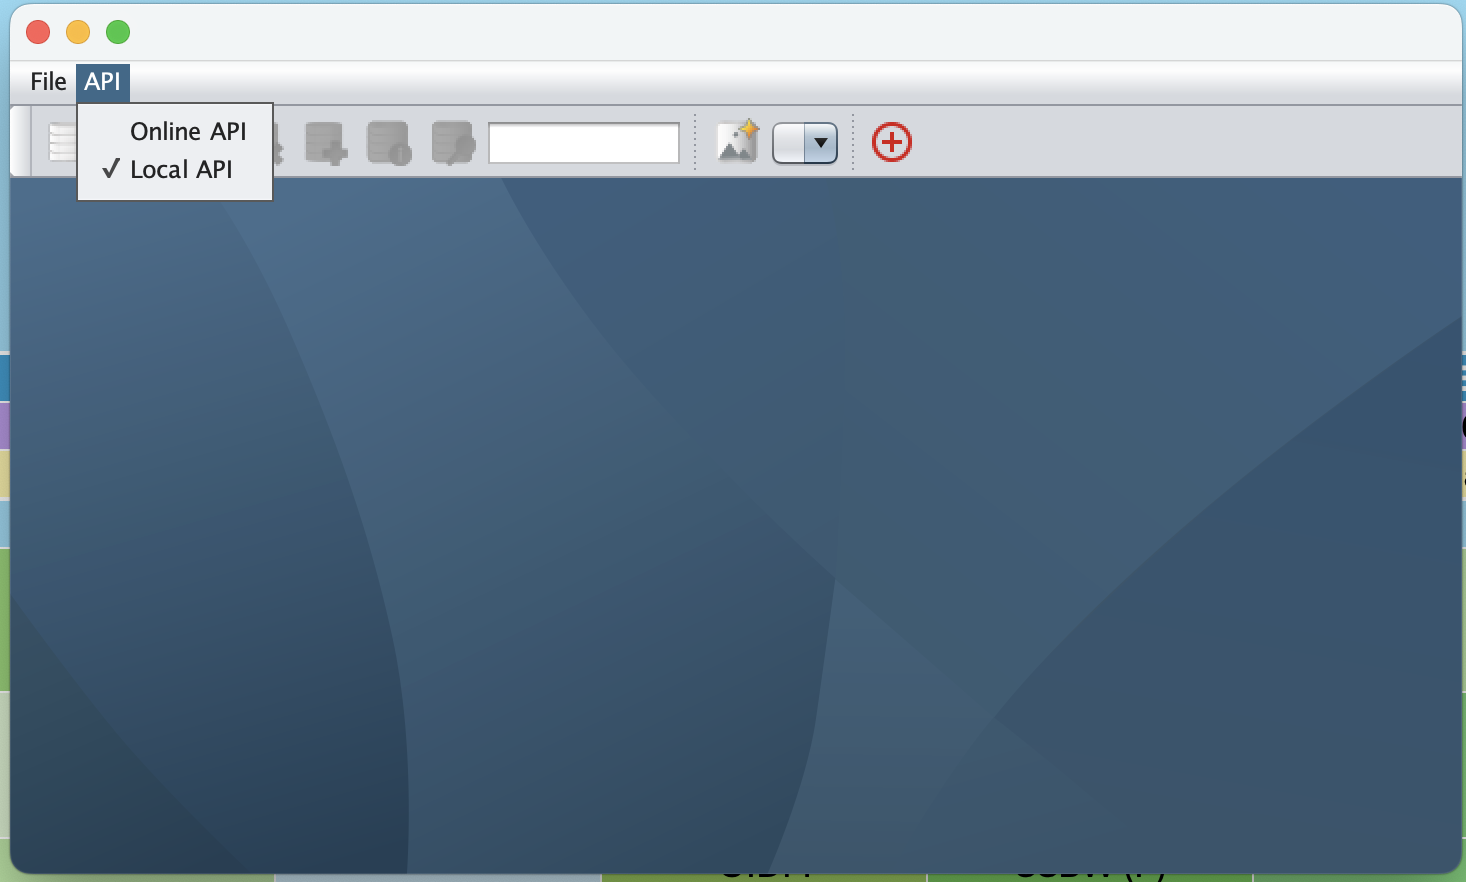
\includegraphics[width=0.5\textwidth]{manual/captura9.png}
\caption{Menú desplegable para seleccionar entre API local u online}
\end{figure}

\paragraph{\textbf{Uso de la Online API}} \mbox{}\\[0.5em]
Si se selecciona la opción \texttt{Online API}, aparecerá un cuadro de diálogo solicitando al usuario que introduzca su \texttt{Hugging Face API Token}.

\begin{itemize}
\item Si se introduce un token válido, el sistema comenzará a utilizar la API online para generar las imágenes.
\item Si se cancela el proceso o se introduce un token vacío, el sistema volverá automáticamente a utilizar la opción \texttt{Local API}.
\end{itemize}

\begin{figure}[H]
\centering
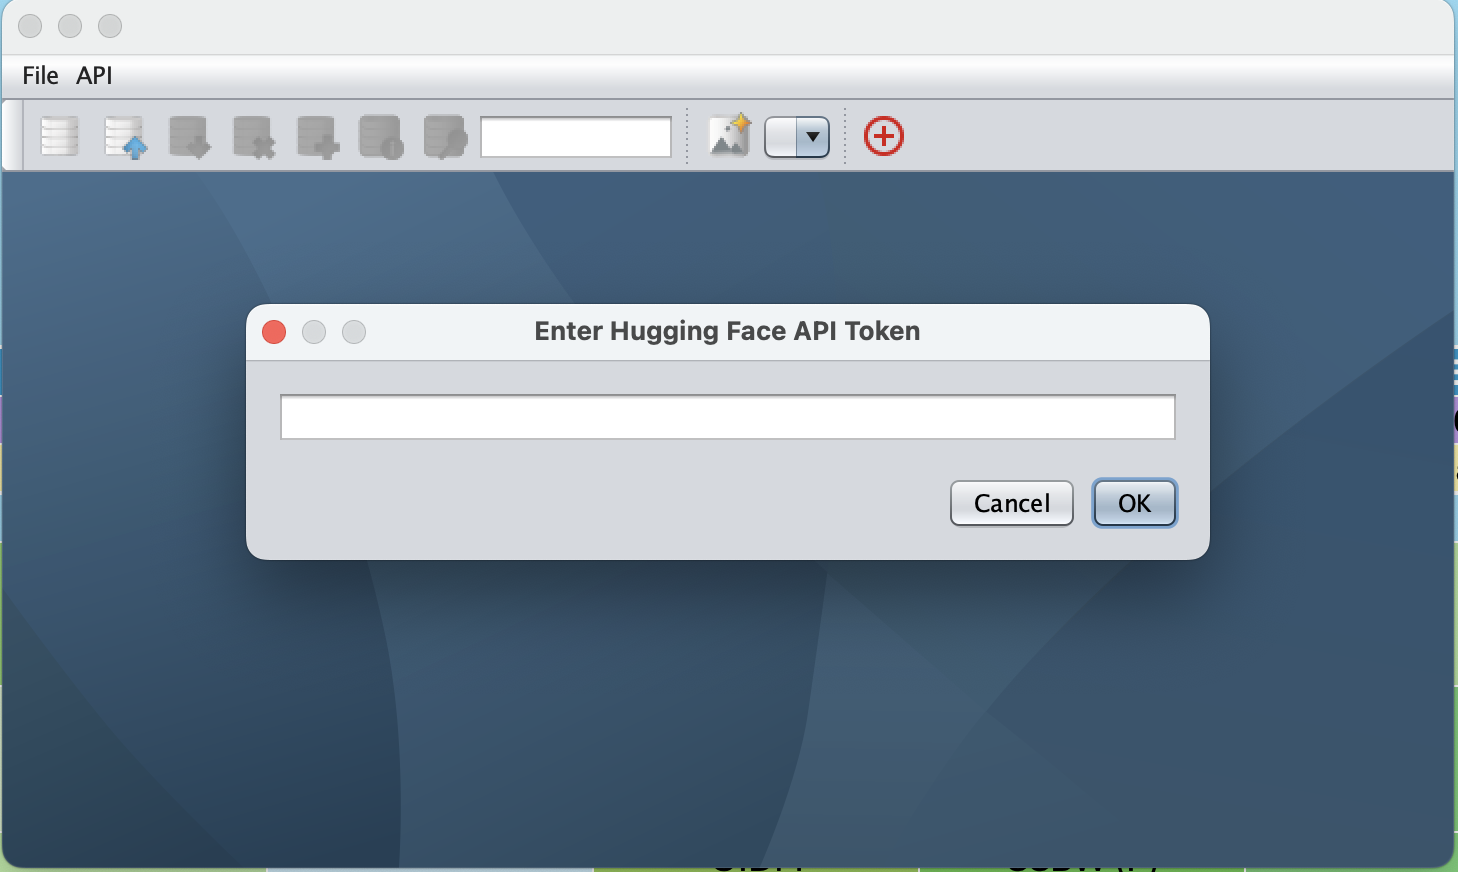
\includegraphics[width=0.5\textwidth]{manual/captura10.png}
\caption{Ventana emergente para introducir el token de Hugging Face}
\end{figure}

\paragraph{\textbf{Consideraciones adicionales}}
\begin{itemize}
\item La elección de API se conserva durante la sesión activa de la aplicación.
\item Se recomienda utilizar la API online solo en entornos con conexión estable y disponer de un token previamente generado desde la plataforma de Hugging Face.
\end{itemize}


\subsection{Cómo generar una imagen}
Para generar una nueva imagen a partir de una descripción textual, sigue los siguientes pasos:
 
\paragraph{\textbf{Paso 1: Acceder al generador}}
\begin{enumerate}
    \item Haz clic en el botón \textit{Generar Imagen}, situado en la barra superior de la aplicación.
    \begin{figure}[H]
        \centering
        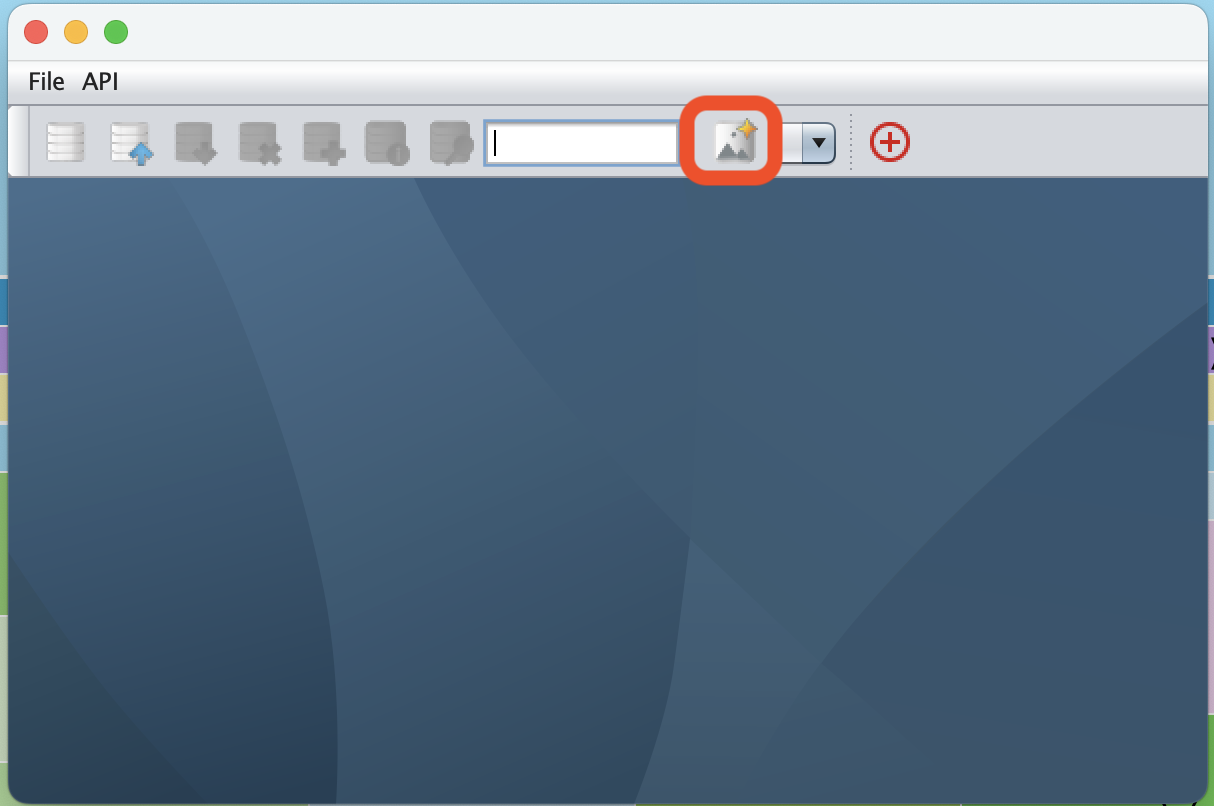
\includegraphics[width=0.45\textwidth]{manual/captura4.png}
        \caption{Botón para generar una imagen}
    \end{figure}

    \item Se abrirá una ventana interna que contiene:
    \begin{itemize}
        \item Un cuadro de texto para introducir la descripción.
        \item Una imagen por defecto como marcador de posición.
        \item Un botón con la etiqueta \textit{Visualizar Imagen}.
    \end{itemize}
    
    \begin{figure}[H]
        \centering
        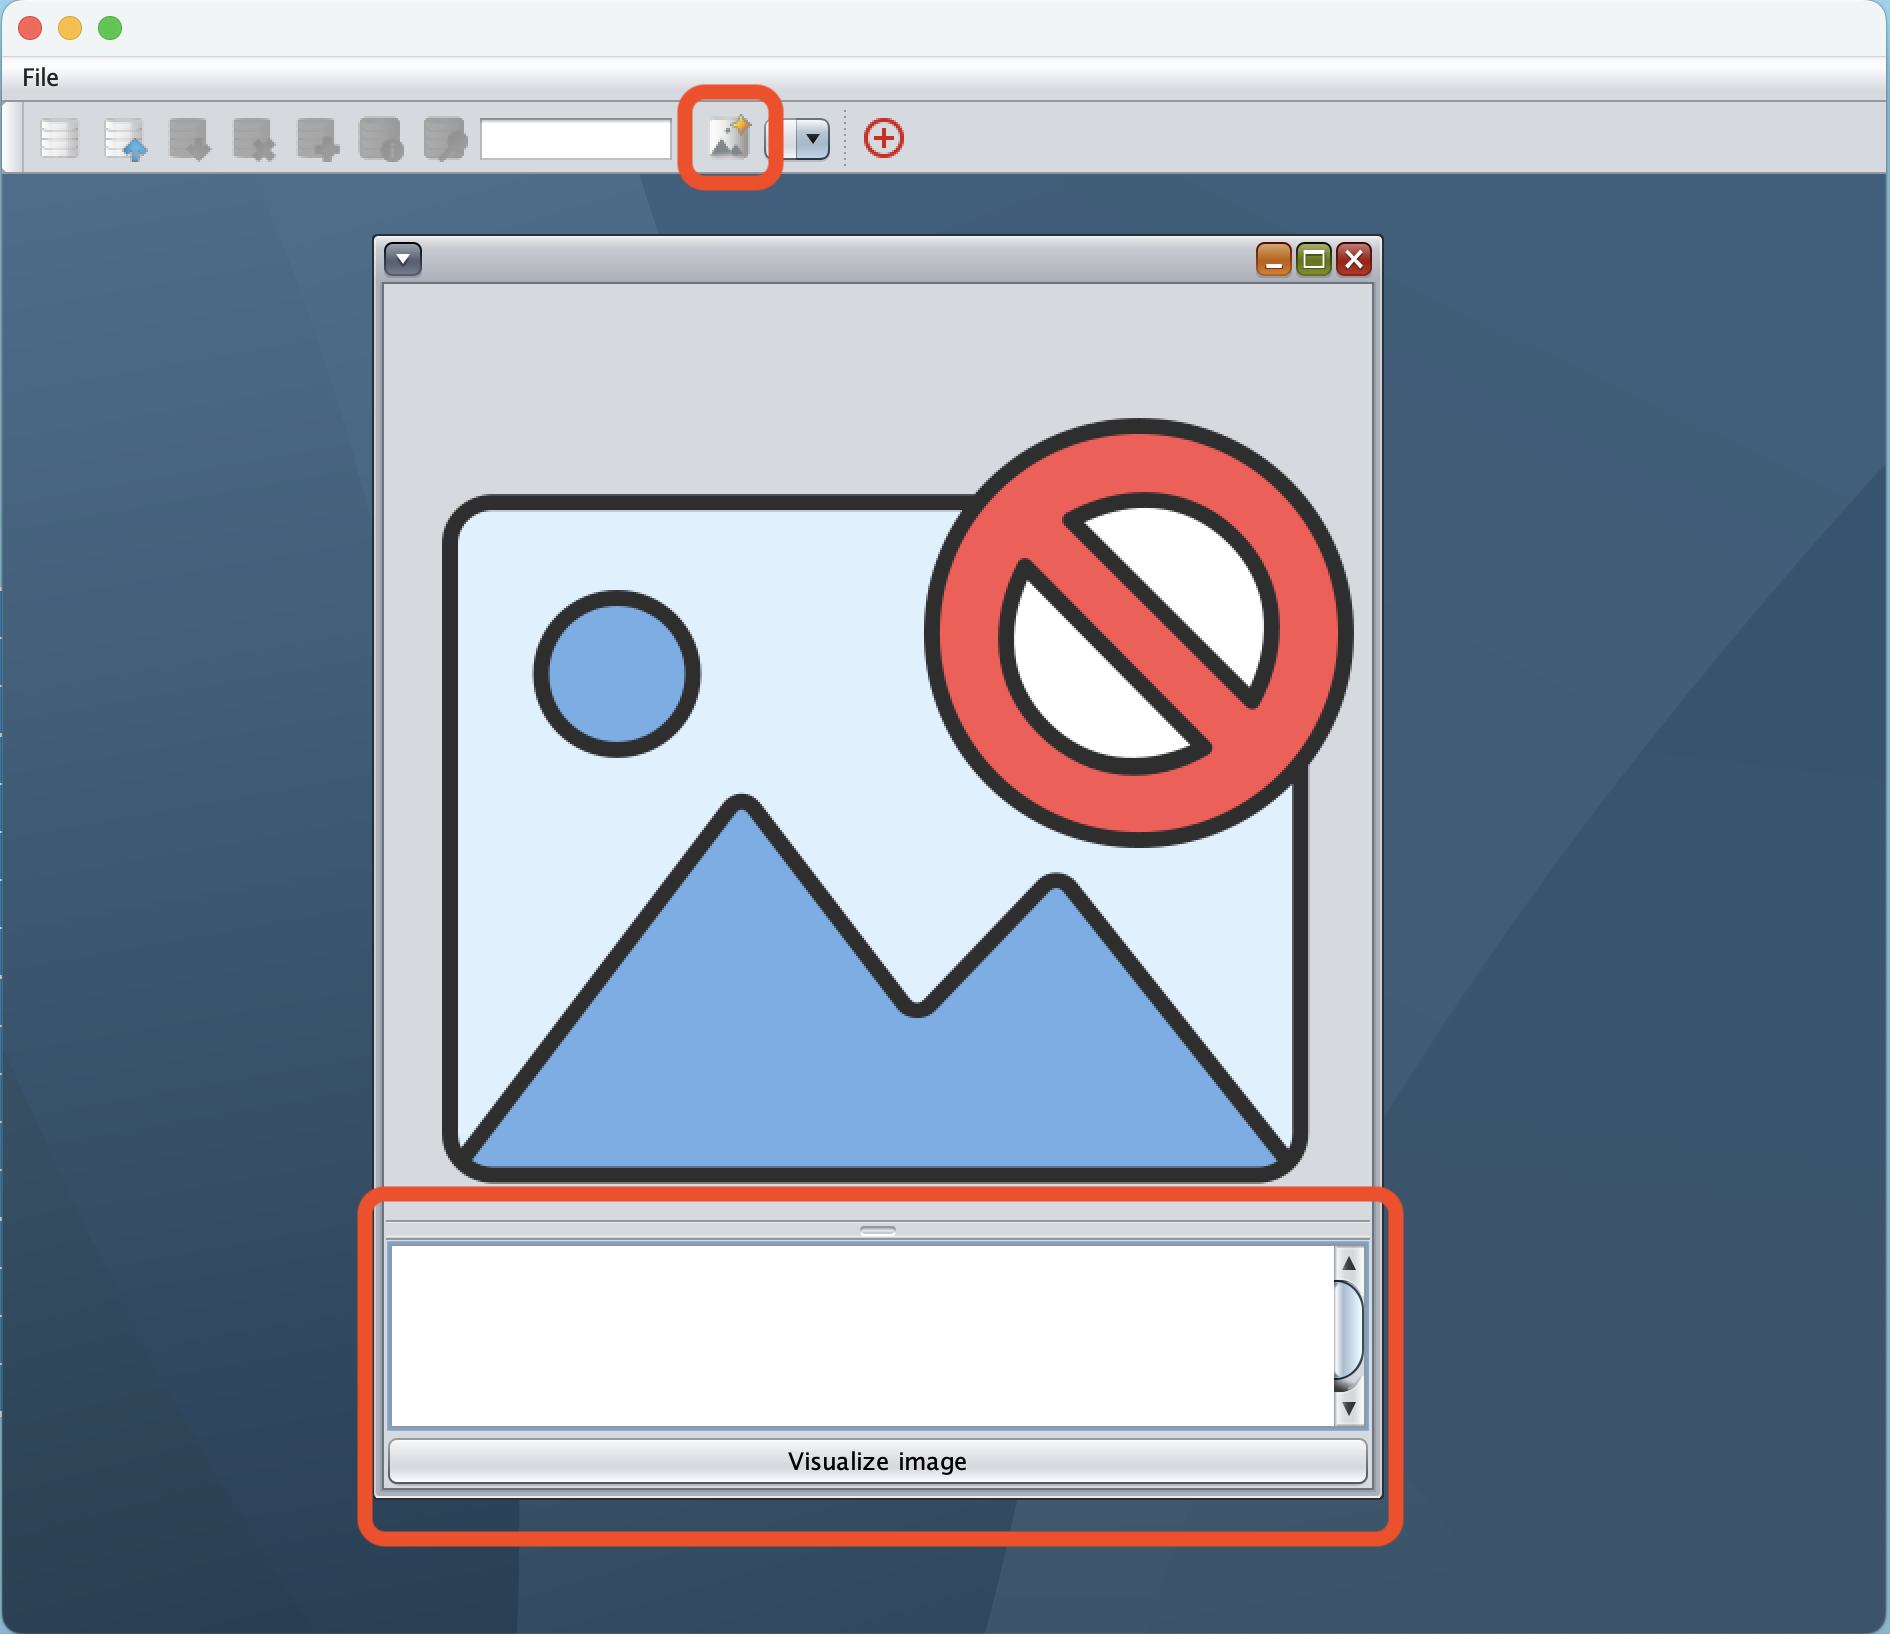
\includegraphics[width=0.45\textwidth]{manual/captura3.png}
        \caption{Ventana interna con área para escribir y botón de visualizar}
    \end{figure}
\end{enumerate}

\textbf{Paso 2: Escribir la descripción}
\begin{enumerate}
    \item En el cuadro de texto, introduce una descripción lo más detallada posible de la imagen que deseas generar.
    \item Ejemplo: \textit{``A dog running on the beach with its friend.''}
\end{enumerate}

    \begin{figure}[H]
        \centering
        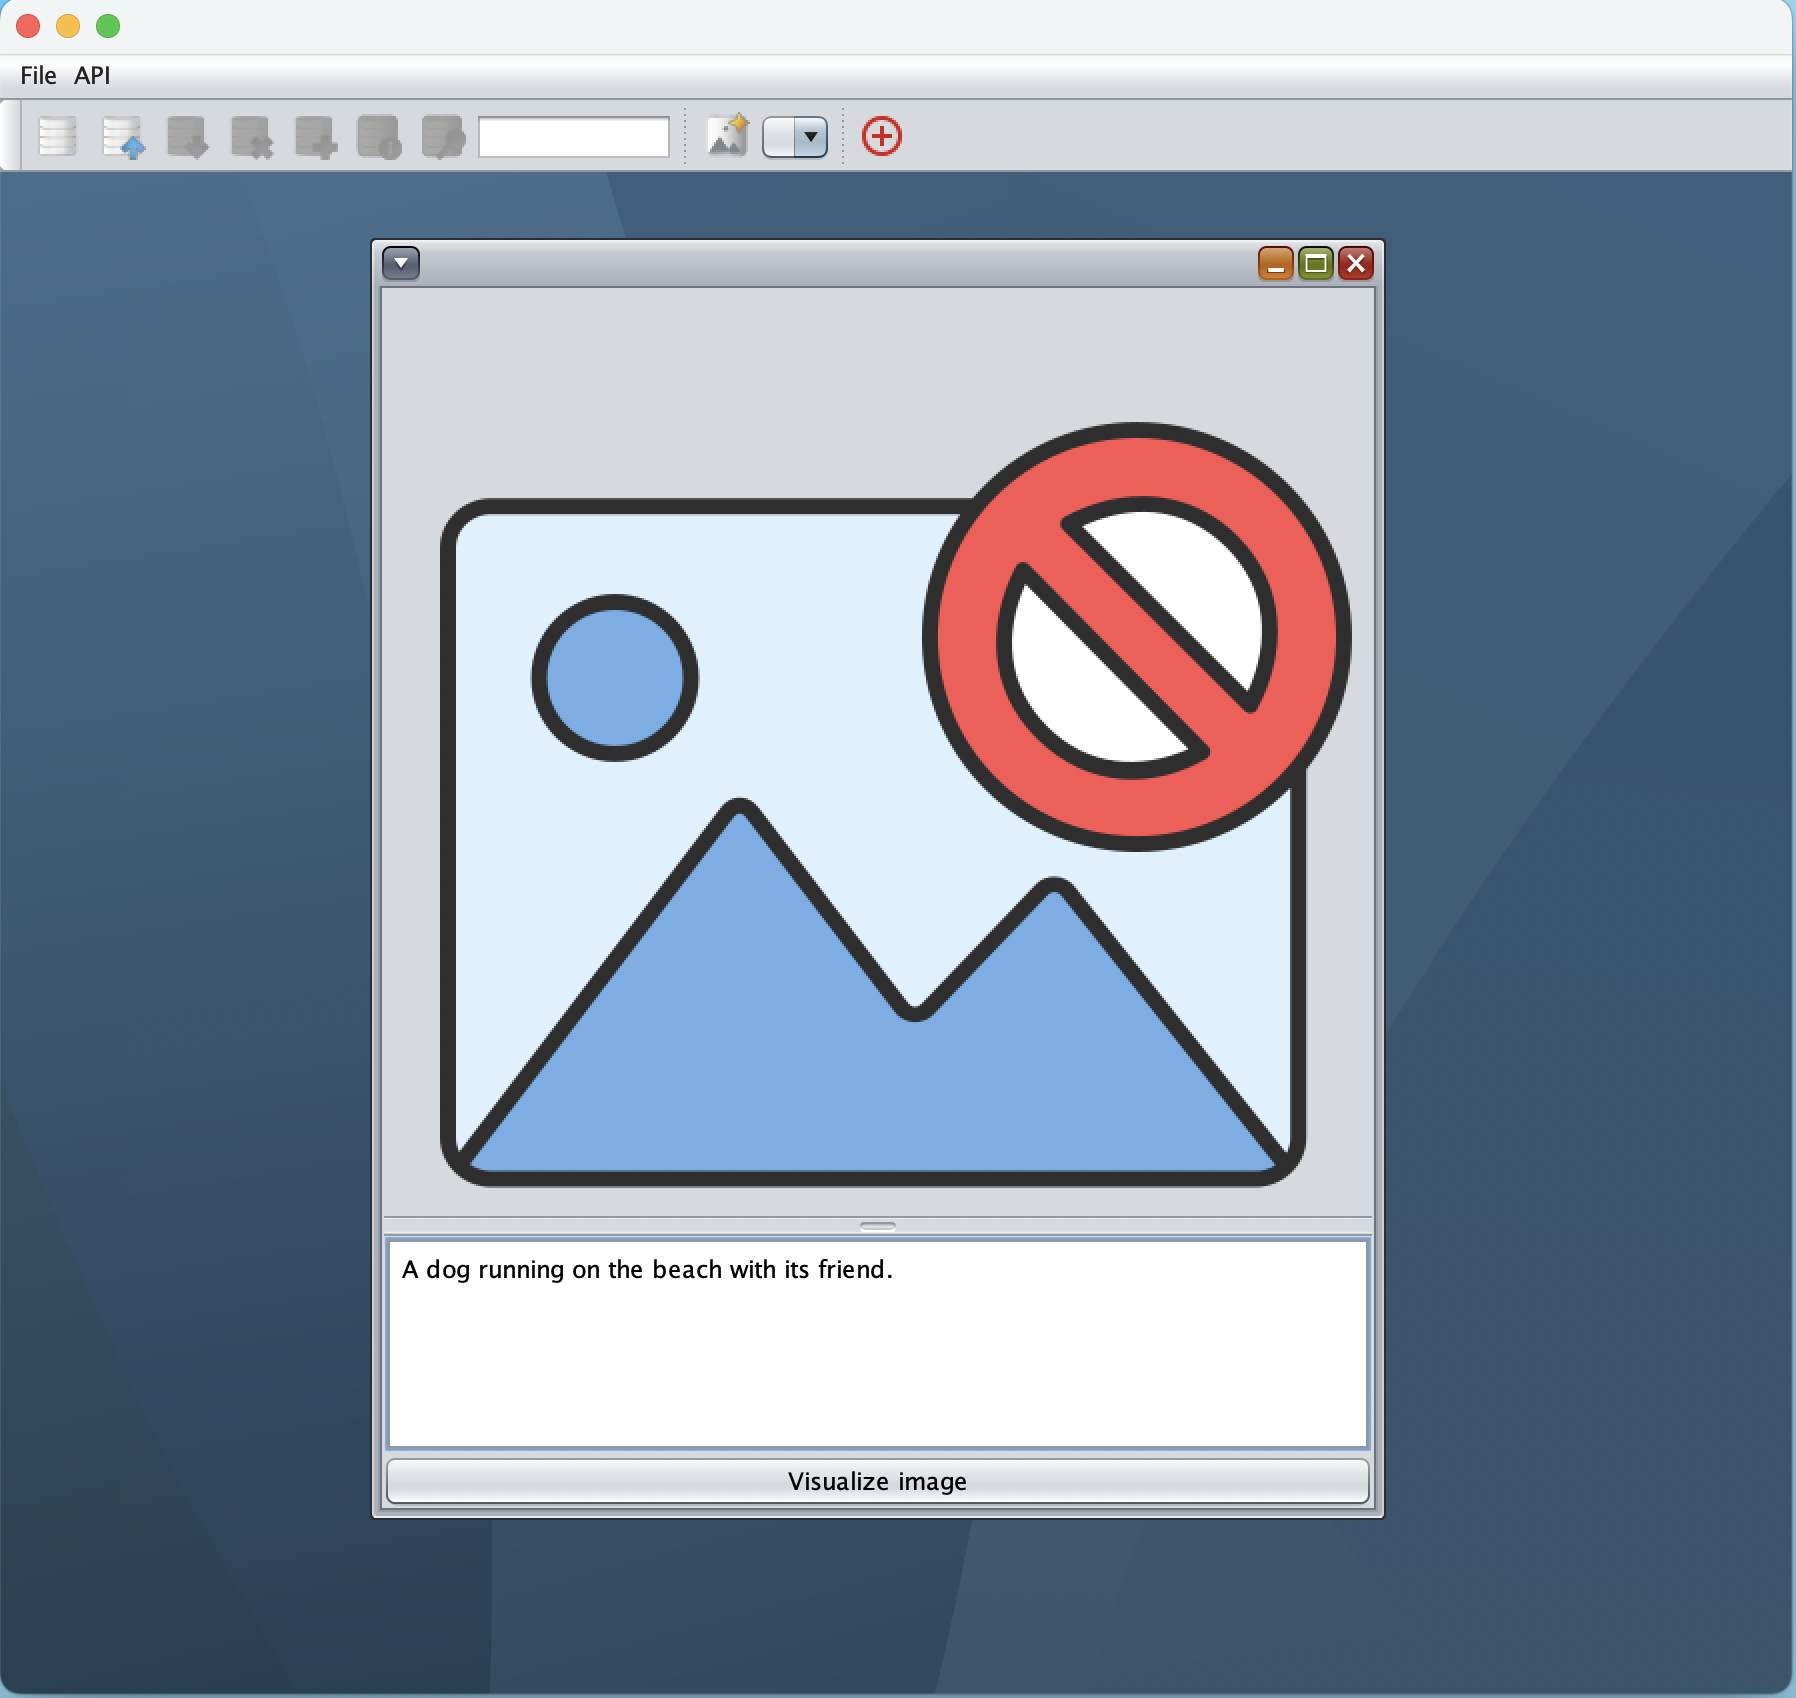
\includegraphics[width=0.5\textwidth]{manual/captura8.png}
        \caption{Ventana interna con área escrita con una descripción de ejemplo}
    \end{figure}

\textbf{Paso 3: Generar y visualizar la imagen}
\begin{enumerate}
    \item Haz clic en el botón \textit{Visualizar Imagen}.
    \item La imagen generada sustituirá a la imagen por defecto en la misma ventana.
    \item Además, la imagen y su descripción se guardarán automáticamente en el historial de generación.
\end{enumerate}

\begin{figure}[H]
    \centering
    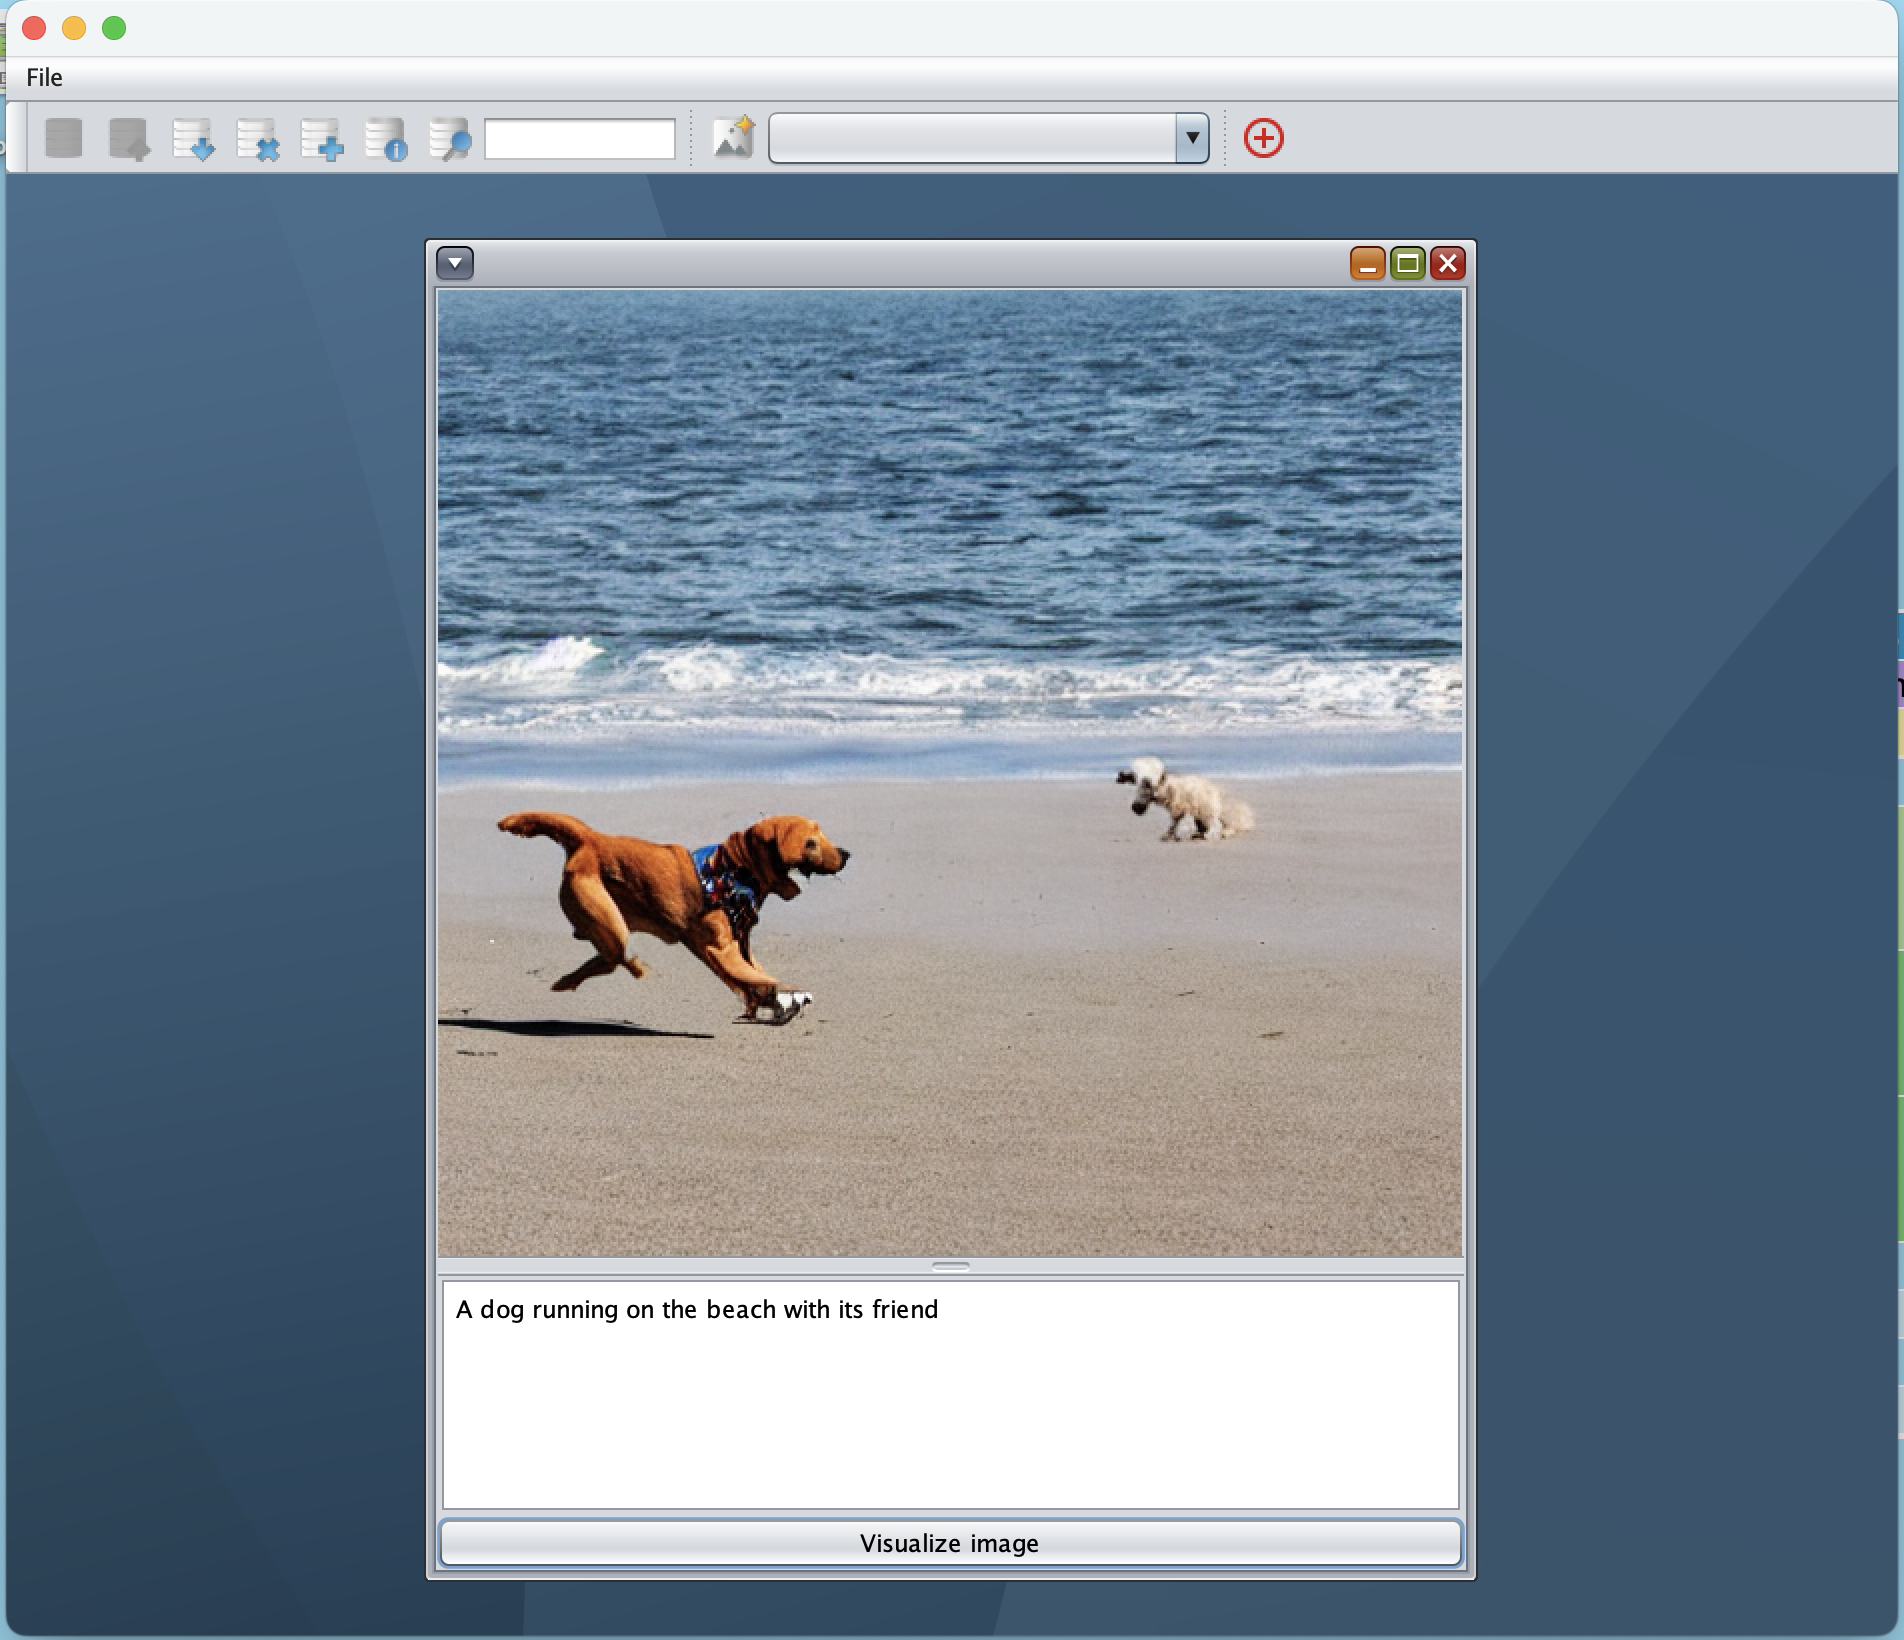
\includegraphics[width=0.5\textwidth]{manual/captura5.png}
    \caption{Ejemplo de visualización}
    \label{fig:ejemplo}
\end{figure}


\subsection{Cómo generar una consulta sin mostrar la imagen}

Esta funcionalidad permite lanzar una consulta basada en una descripción textual sin necesidad de generar ni visualizar la imagen en pantalla. En su lugar, se realiza una búsqueda en la base de datos para recuperar resultados visualmente similares.

\paragraph{\textbf{Paso 1: Escribir la descripción}}
\begin{enumerate}
    \item Introduce el texto descriptivo en el cuadro situado en la barra de herramientas superior.
    \item Ejemplo: \textit{``A lot of colorful sprinkles."}
\end{enumerate}

\begin{figure}[H]
    \centering
    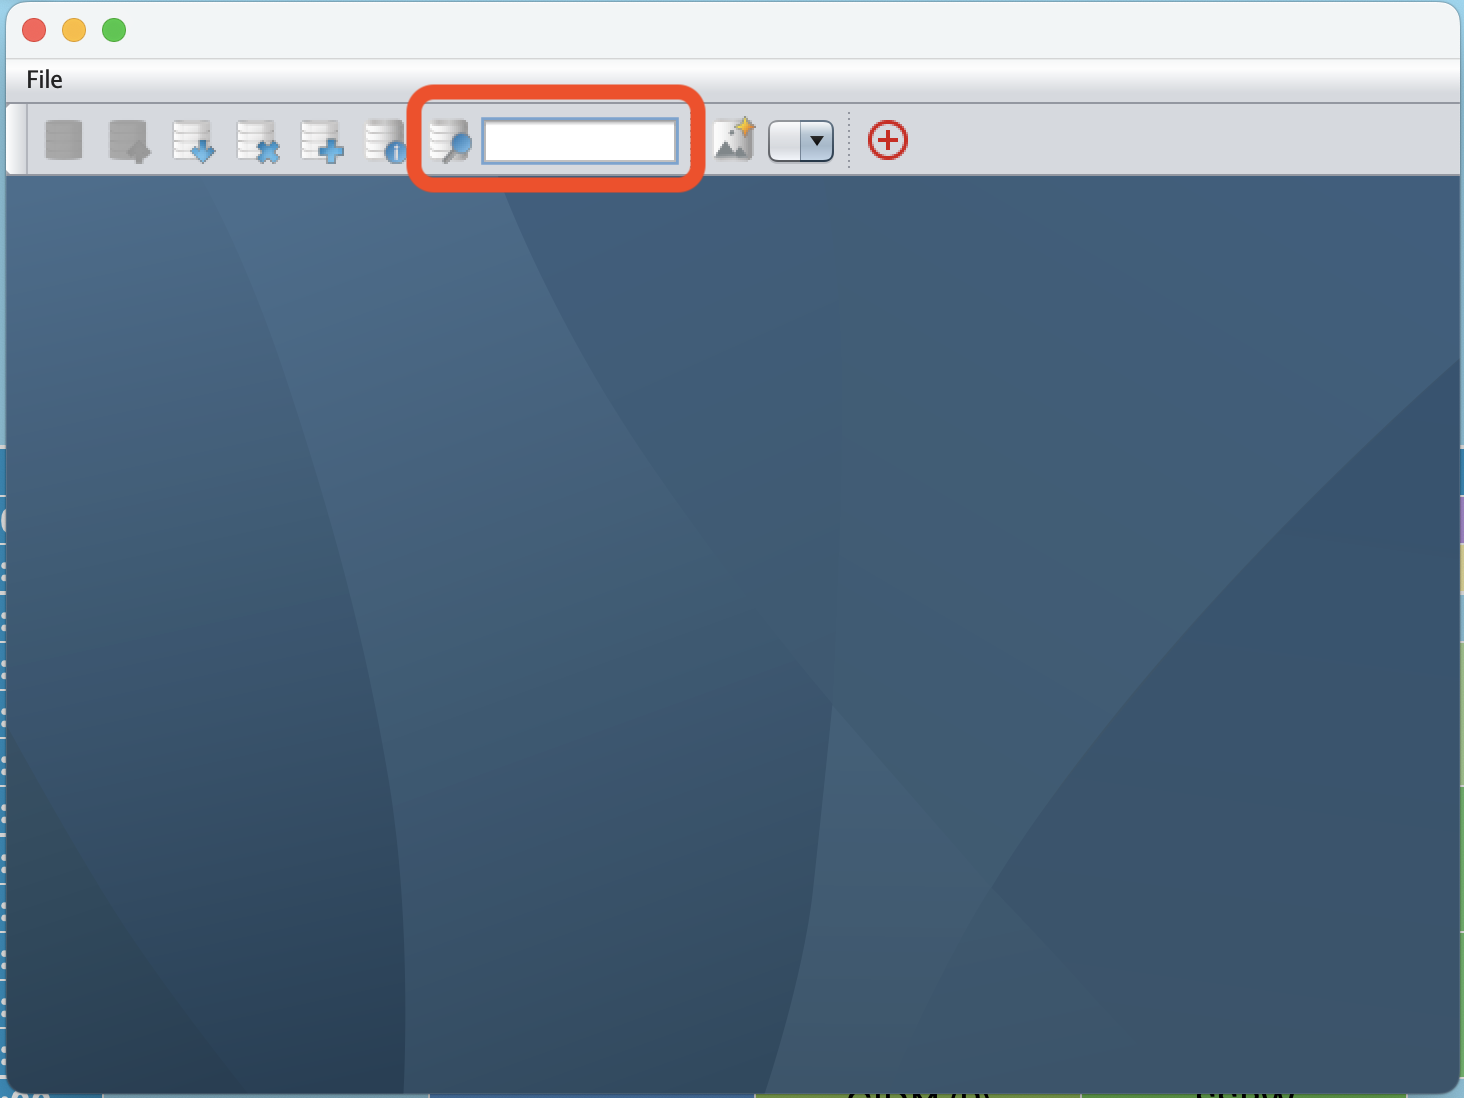
\includegraphics[width=0.5\textwidth]{manual/captura2.png}
    \caption{Escribir la descripción en la barra superior}
    \label{fig:consulta-cuadro}
\end{figure}

\paragraph{\textbf{Paso 2: Ejecutar la consulta}}
\begin{enumerate}
    \item Haz clic en el botón de búsqueda situado junto al cuadro de texto.
    \item El sistema generará la imagen en segundo plano y lanzará una búsqueda automática en la base de datos utilizando la imagen como consulta.
\end{enumerate}

\begin{figure}[H]
    \centering
    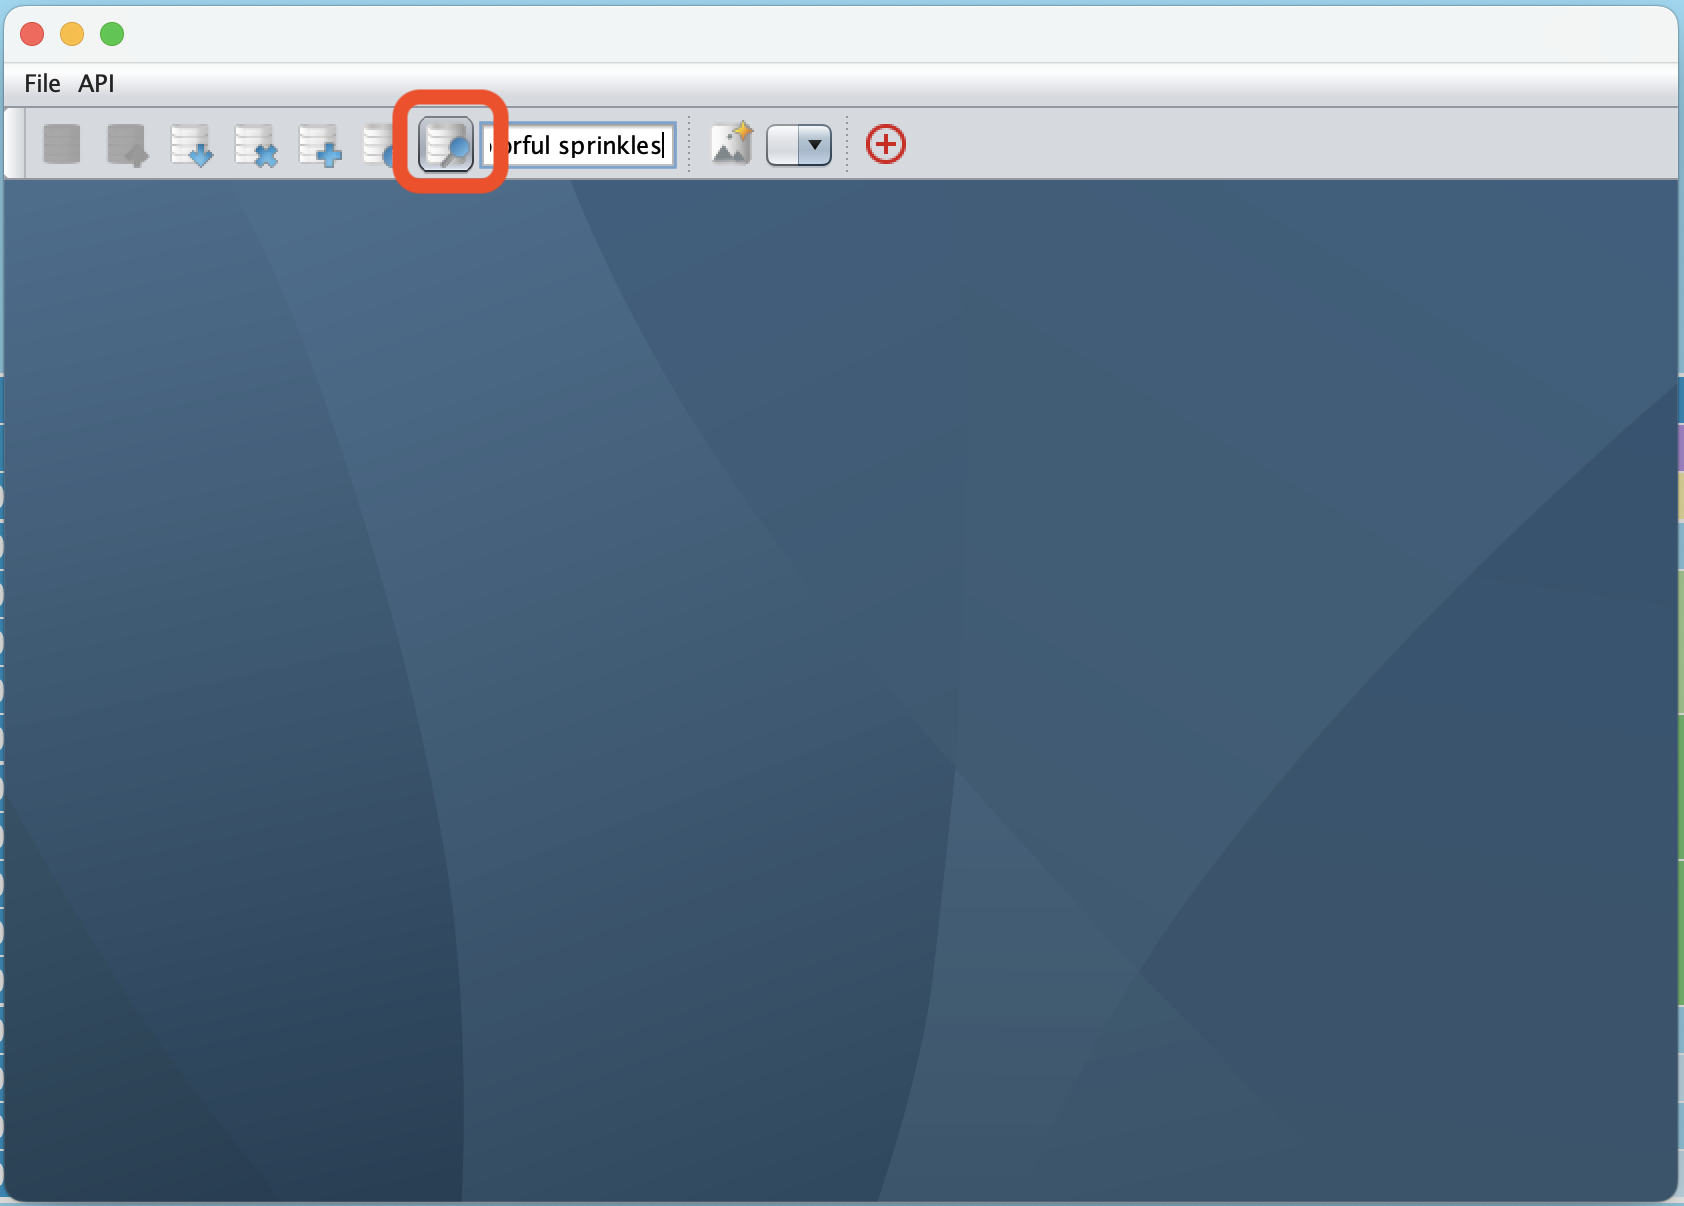
\includegraphics[width=0.5\textwidth]{manual/captura11.png}
    \caption{Botón de búsqueda para ejecutar la consulta}
\end{figure}


\paragraph{\textbf{Paso 3: Visualización de resultados}}
\begin{enumerate}
    \item Se abrirá una nueva ventana con los resultados visuales recuperados desde la base de datos, similares a la imagen generada a partir de tu descripción.
\end{enumerate}

\begin{figure}[H]
    \centering
    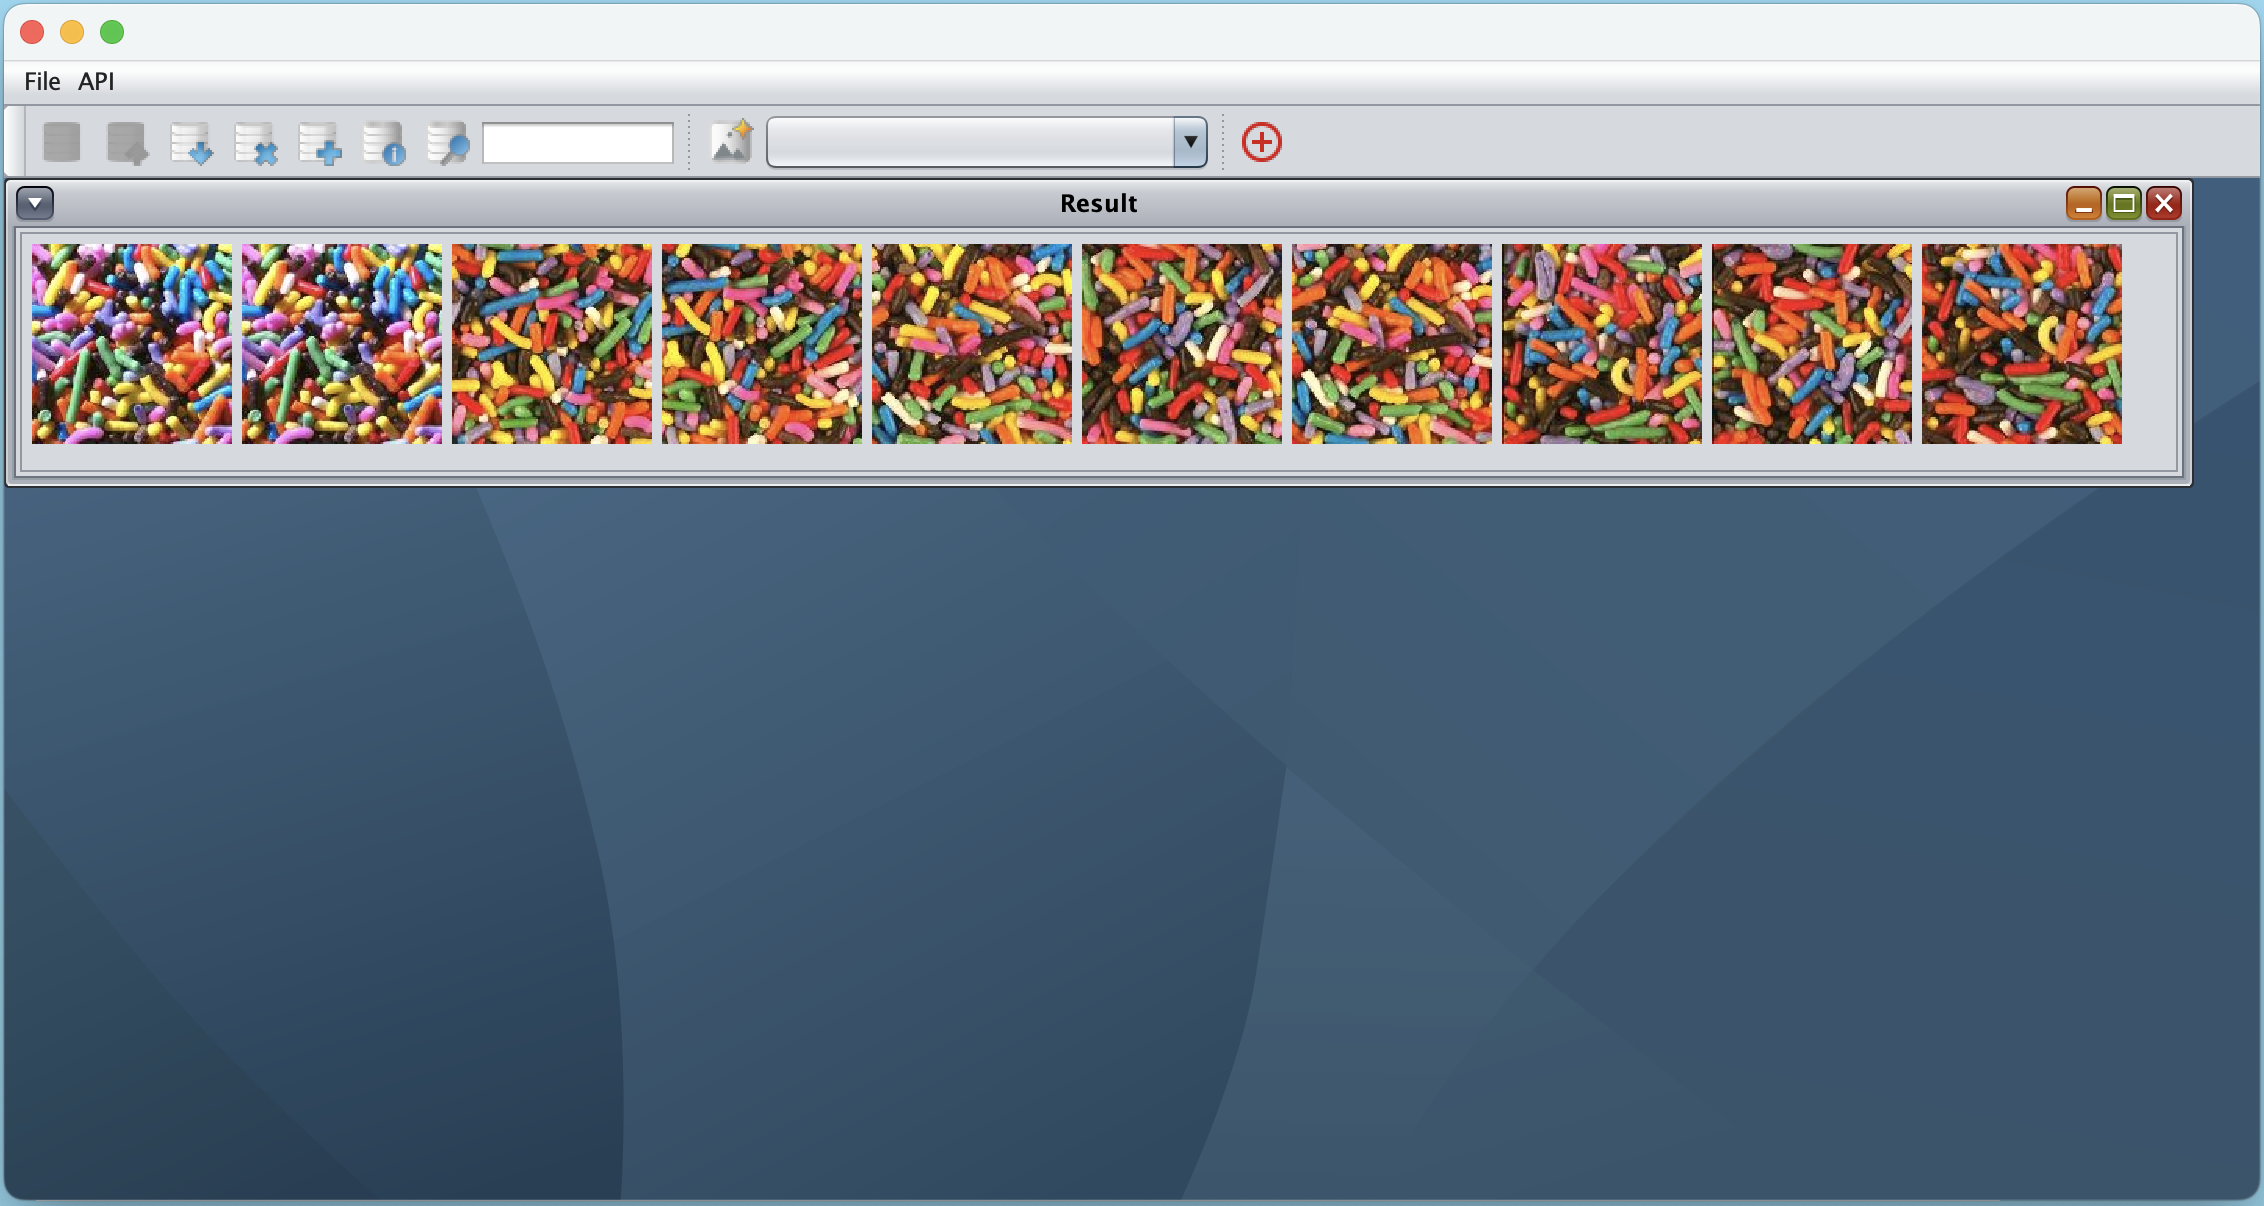
\includegraphics[width=0.5\textwidth]{manual/captura12.png}
    \caption{Resultados visuales recuperados de la base de datos}
\end{figure}

\subsection{Reutilizar imágenes generadas}
Todas las imágenes generadas se almacenan automáticamente en el historial, junto con la descripción (prompt) que se utilizó para crearlas. Este historial se encuentra accesible mediante una lista desplegable en la parte superior de la interfaz.

Para reutilizar una imagen generada anteriormente:
\begin{enumerate}
    \item Despliega la lista situada en la parte superior.
    \item Selecciona una de las entradas del historial (aparecen truncadas si son largas, pero se muestran completas en su tooltip).
    \item La imagen correspondiente se abrirá en una nueva ventana interna, con el texto de la descripción como título.
\end{enumerate}

\begin{figure}[H]
    \centering
    \begin{minipage}[t]{0.48\textwidth}
        \centering
        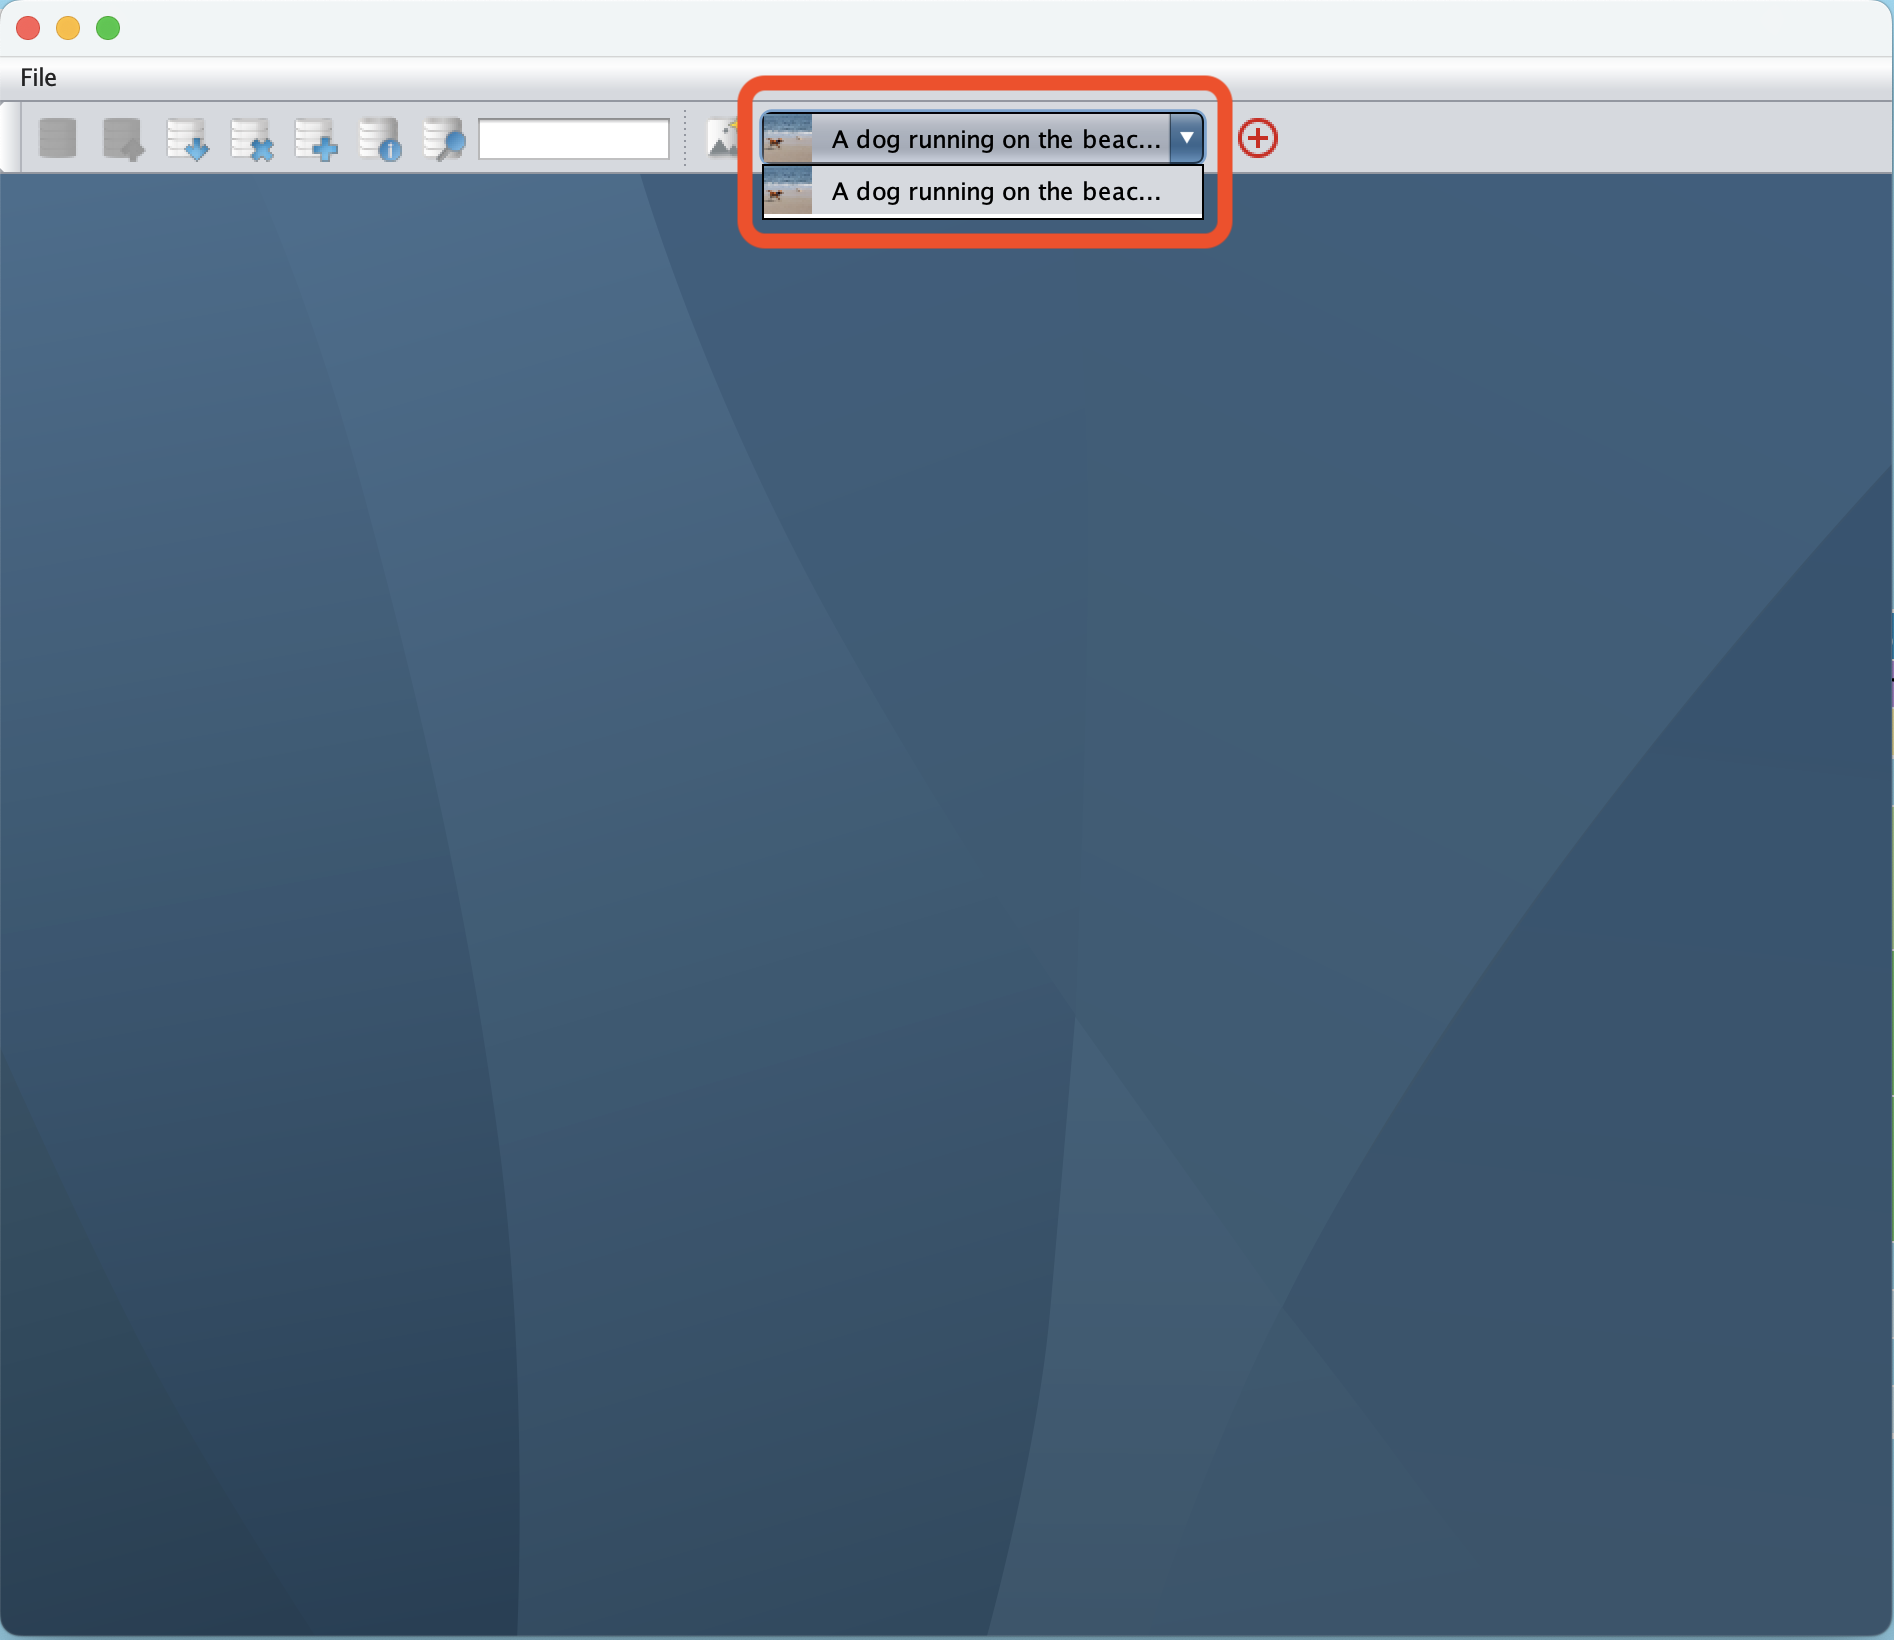
\includegraphics[width=\textwidth]{manual/captura6.png}
    \end{minipage}
    \hfill
    \begin{minipage}[t]{0.48\textwidth}
        \centering
        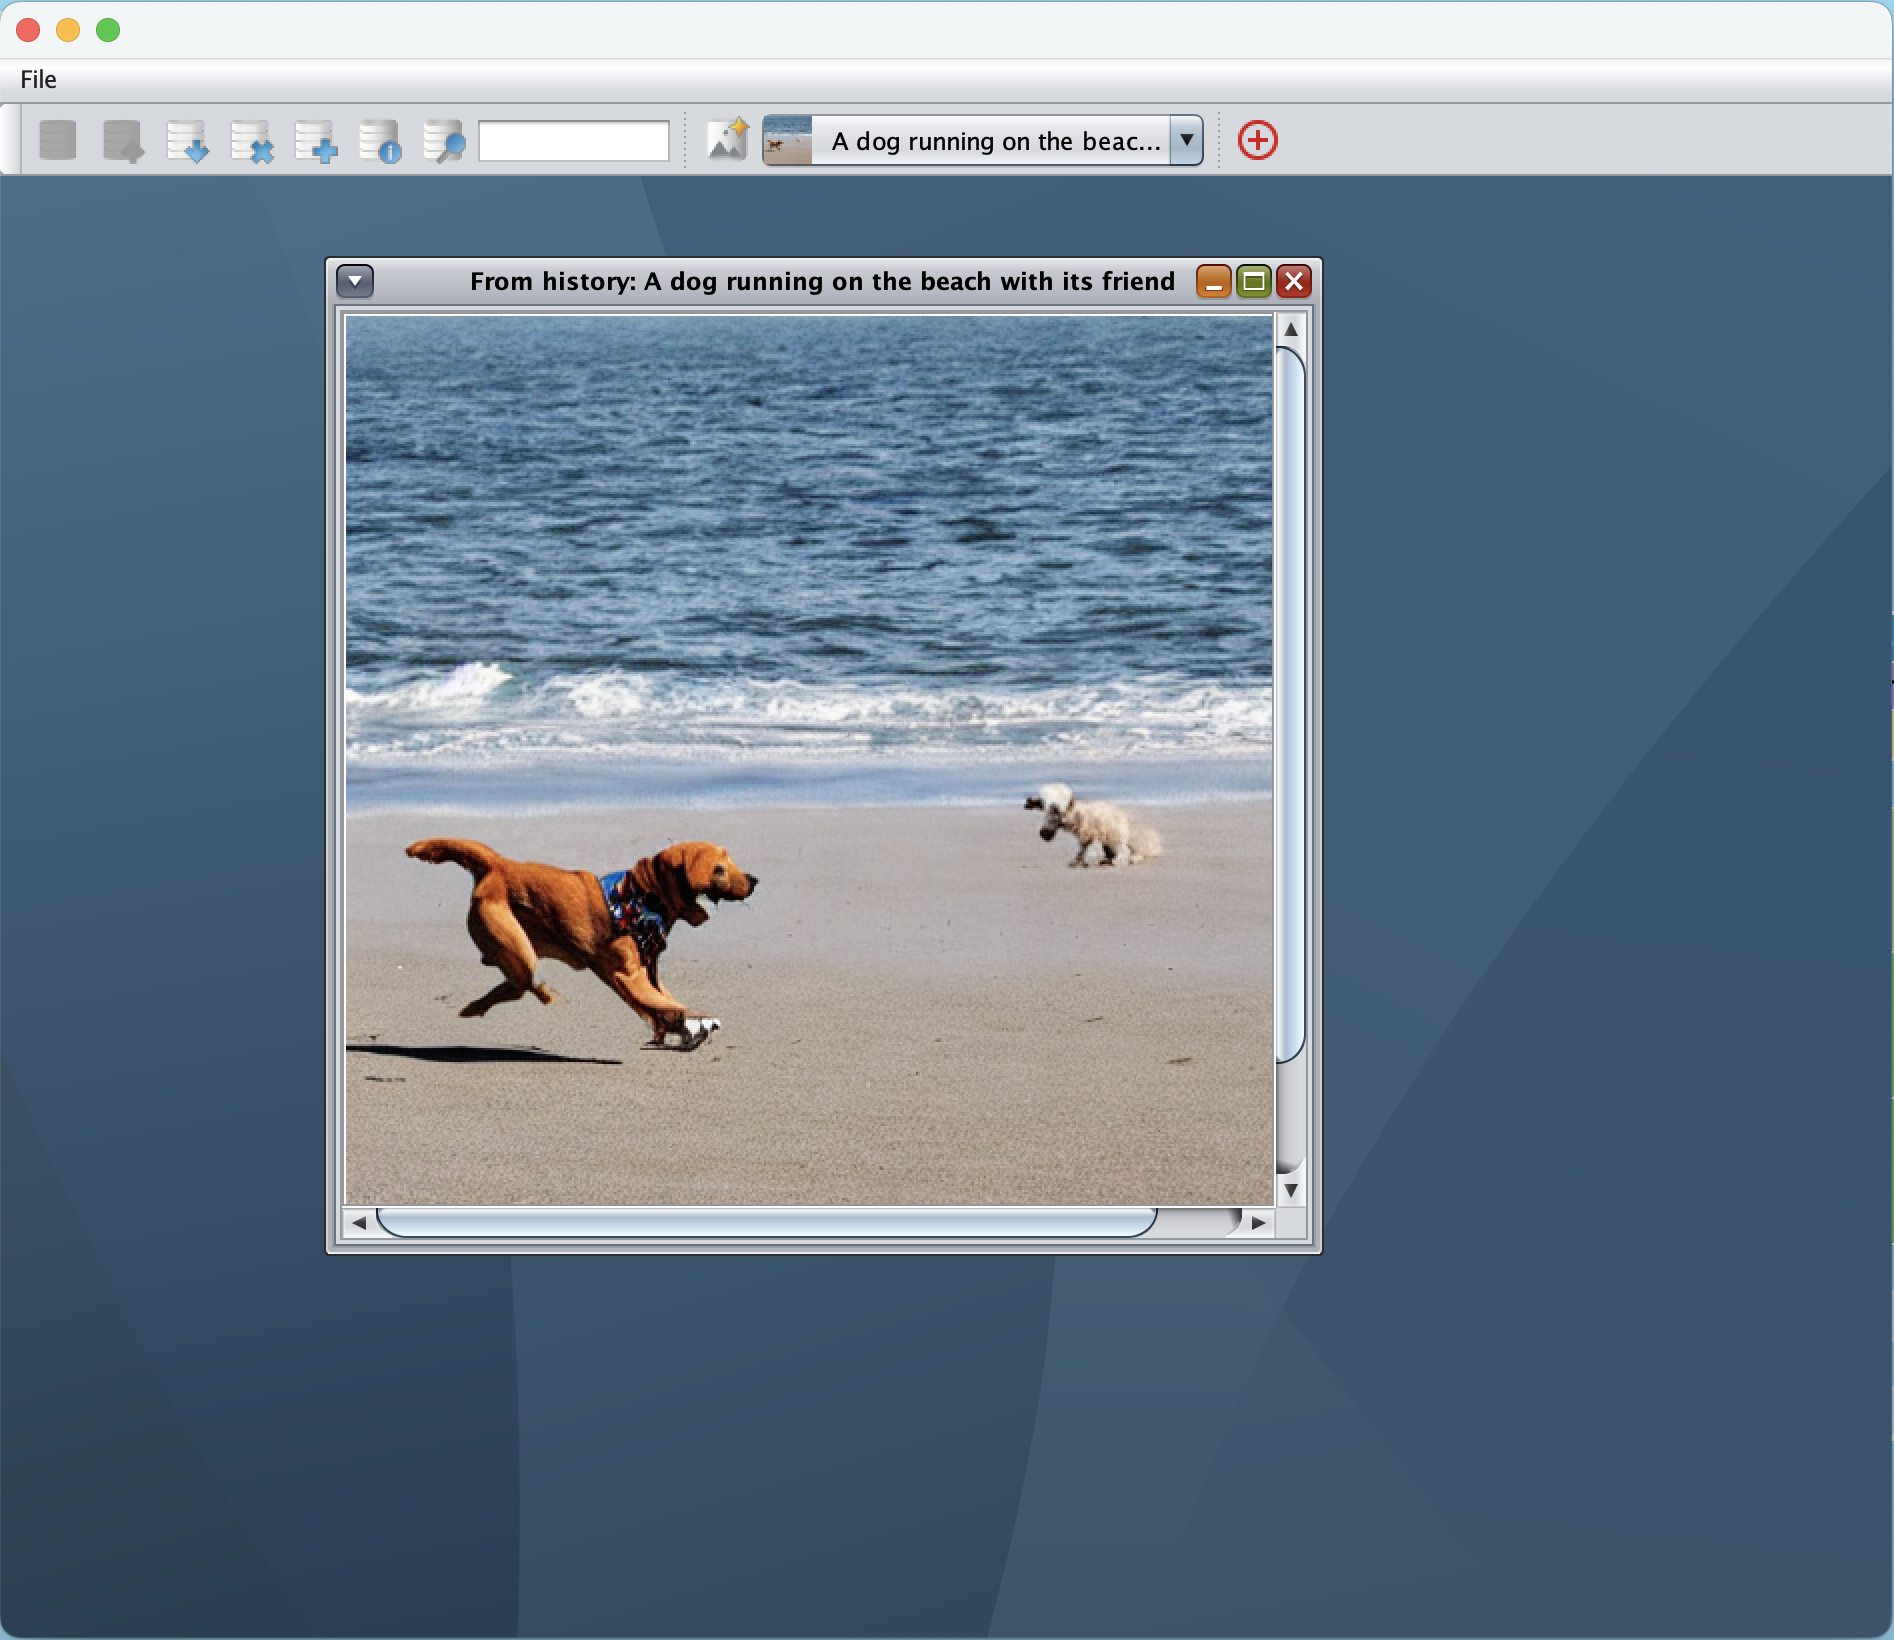
\includegraphics[width=\textwidth]{manual/captura7.png}
    \end{minipage}
    \caption{A la izquierda, vista del historial con una entrada seleccionada. A la derecha, la imagen generada que se abre al seleccionar esa entrada.}
    \label{fig:historial}
\end{figure}


\subsection{Errores y soluciones comunes}

Durante el uso del sistema, pueden producirse ciertos errores que impidan temporalmente la generación de imágenes o la interacción con algunos elementos de la interfaz. A continuación se describen los más frecuentes y las acciones recomendadas para resolverlos:

\begin{itemize}
\item \textbf{Error al generar la imagen}
\begin{itemize}
\item \textbf{Mensaje:} ``No se pudo generar la imagen. Verifique su descripción.''
\item \textbf{Causa:} El prompt puede estar vacío o ser demasiado ambiguo.
\item \textbf{Solución:} Introduce una descripción más detallada y coherente. Por ejemplo, en lugar de escribir \textit{“un animal”}, puedes escribir \textit{“a cat with green eyes sitting on a sofa”}.
\end{itemize}
\item \textbf{Error al cargar el modelo}  
\begin{itemize}
    \item \textbf{Mensaje:} ``El modelo seleccionado no es compatible.''
    \item \textbf{Causa:} Se ha cargado un archivo ZIP con estructura incorrecta o faltan archivos esenciales del modelo.
    \item \textbf{Solución:} Asegúrate de que el ZIP contenga los archivos requeridos como \texttt{config.json}, \texttt{model.safetensors}, \texttt{tokenizer\_config.json}, etc. Utiliza modelos que hayan sido exportados siguiendo el formato esperado por la API.
\end{itemize}

\item \textbf{Error de conexión al utilizar la API online}  
\begin{itemize}
    \item \textbf{Mensaje:} ``Error de autenticación con la API. Token inválido o expirado.''
    \item \textbf{Causa:} El token de Hugging Face es incorrecto o ha caducado.
    \item \textbf{Solución:} Verifica que has introducido el token correctamente. Puedes generar un nuevo token accediendo a tu cuenta en [https://huggingface.co/settings/tokens].
\end{itemize}

\item \textbf{Error de red al generar con API online}  
\begin{itemize}
    \item \textbf{Mensaje:} ``No se pudo contactar con el servidor de generación de imágenes.''
    \item \textbf{Causa:} Falta de conexión a Internet o fallo del servidor externo.
    \item \textbf{Solución:} Comprueba tu conexión a Internet. En caso de persistir el error, cambia temporalmente a la opción \texttt{Local API} desde el menú superior.
\end{itemize}

\item \textbf{Error al abrir una imagen desde el historial}  
\begin{itemize}
    \item \textbf{Mensaje:} ``La imagen seleccionada no se encuentra disponible.''
    \item \textbf{Causa:} El archivo correspondiente ha sido eliminado o movido manualmente.
    \item \textbf{Solución:} Evita modificar directamente la carpeta donde se almacenan las imágenes generadas. Si necesitas liberar espacio, utiliza la función de limpieza integrada en versiones futuras.
\end{itemize}
\end{itemize}

\vspace{1em}
Para cualquier otro error no contemplado aquí, se recomienda reiniciar la aplicación y consultar la documentación técnica o contactar con el equipo de soporte.